% Options for packages loaded elsewhere
\PassOptionsToPackage{unicode}{hyperref}
\PassOptionsToPackage{hyphens}{url}
%
\documentclass[
  11pt,
]{article}
\usepackage{amsmath,amssymb}
\usepackage{lmodern}
\usepackage{iftex}
\ifPDFTeX
  \usepackage[T1]{fontenc}
  \usepackage[utf8]{inputenc}
  \usepackage{textcomp} % provide euro and other symbols
\else % if luatex or xetex
  \usepackage{unicode-math}
  \defaultfontfeatures{Scale=MatchLowercase}
  \defaultfontfeatures[\rmfamily]{Ligatures=TeX,Scale=1}
\fi
% Use upquote if available, for straight quotes in verbatim environments
\IfFileExists{upquote.sty}{\usepackage{upquote}}{}
\IfFileExists{microtype.sty}{% use microtype if available
  \usepackage[]{microtype}
  \UseMicrotypeSet[protrusion]{basicmath} % disable protrusion for tt fonts
}{}
\makeatletter
\@ifundefined{KOMAClassName}{% if non-KOMA class
  \IfFileExists{parskip.sty}{%
    \usepackage{parskip}
  }{% else
    \setlength{\parindent}{0pt}
    \setlength{\parskip}{6pt plus 2pt minus 1pt}}
}{% if KOMA class
  \KOMAoptions{parskip=half}}
\makeatother
\usepackage{xcolor}
\usepackage[margin=1in]{geometry}
\usepackage{color}
\usepackage{fancyvrb}
\newcommand{\VerbBar}{|}
\newcommand{\VERB}{\Verb[commandchars=\\\{\}]}
\DefineVerbatimEnvironment{Highlighting}{Verbatim}{commandchars=\\\{\}}
% Add ',fontsize=\small' for more characters per line
\usepackage{framed}
\definecolor{shadecolor}{RGB}{248,248,248}
\newenvironment{Shaded}{\begin{snugshade}}{\end{snugshade}}
\newcommand{\AlertTok}[1]{\textcolor[rgb]{0.94,0.16,0.16}{#1}}
\newcommand{\AnnotationTok}[1]{\textcolor[rgb]{0.56,0.35,0.01}{\textbf{\textit{#1}}}}
\newcommand{\AttributeTok}[1]{\textcolor[rgb]{0.77,0.63,0.00}{#1}}
\newcommand{\BaseNTok}[1]{\textcolor[rgb]{0.00,0.00,0.81}{#1}}
\newcommand{\BuiltInTok}[1]{#1}
\newcommand{\CharTok}[1]{\textcolor[rgb]{0.31,0.60,0.02}{#1}}
\newcommand{\CommentTok}[1]{\textcolor[rgb]{0.56,0.35,0.01}{\textit{#1}}}
\newcommand{\CommentVarTok}[1]{\textcolor[rgb]{0.56,0.35,0.01}{\textbf{\textit{#1}}}}
\newcommand{\ConstantTok}[1]{\textcolor[rgb]{0.00,0.00,0.00}{#1}}
\newcommand{\ControlFlowTok}[1]{\textcolor[rgb]{0.13,0.29,0.53}{\textbf{#1}}}
\newcommand{\DataTypeTok}[1]{\textcolor[rgb]{0.13,0.29,0.53}{#1}}
\newcommand{\DecValTok}[1]{\textcolor[rgb]{0.00,0.00,0.81}{#1}}
\newcommand{\DocumentationTok}[1]{\textcolor[rgb]{0.56,0.35,0.01}{\textbf{\textit{#1}}}}
\newcommand{\ErrorTok}[1]{\textcolor[rgb]{0.64,0.00,0.00}{\textbf{#1}}}
\newcommand{\ExtensionTok}[1]{#1}
\newcommand{\FloatTok}[1]{\textcolor[rgb]{0.00,0.00,0.81}{#1}}
\newcommand{\FunctionTok}[1]{\textcolor[rgb]{0.00,0.00,0.00}{#1}}
\newcommand{\ImportTok}[1]{#1}
\newcommand{\InformationTok}[1]{\textcolor[rgb]{0.56,0.35,0.01}{\textbf{\textit{#1}}}}
\newcommand{\KeywordTok}[1]{\textcolor[rgb]{0.13,0.29,0.53}{\textbf{#1}}}
\newcommand{\NormalTok}[1]{#1}
\newcommand{\OperatorTok}[1]{\textcolor[rgb]{0.81,0.36,0.00}{\textbf{#1}}}
\newcommand{\OtherTok}[1]{\textcolor[rgb]{0.56,0.35,0.01}{#1}}
\newcommand{\PreprocessorTok}[1]{\textcolor[rgb]{0.56,0.35,0.01}{\textit{#1}}}
\newcommand{\RegionMarkerTok}[1]{#1}
\newcommand{\SpecialCharTok}[1]{\textcolor[rgb]{0.00,0.00,0.00}{#1}}
\newcommand{\SpecialStringTok}[1]{\textcolor[rgb]{0.31,0.60,0.02}{#1}}
\newcommand{\StringTok}[1]{\textcolor[rgb]{0.31,0.60,0.02}{#1}}
\newcommand{\VariableTok}[1]{\textcolor[rgb]{0.00,0.00,0.00}{#1}}
\newcommand{\VerbatimStringTok}[1]{\textcolor[rgb]{0.31,0.60,0.02}{#1}}
\newcommand{\WarningTok}[1]{\textcolor[rgb]{0.56,0.35,0.01}{\textbf{\textit{#1}}}}
\usepackage{graphicx}
\makeatletter
\def\maxwidth{\ifdim\Gin@nat@width>\linewidth\linewidth\else\Gin@nat@width\fi}
\def\maxheight{\ifdim\Gin@nat@height>\textheight\textheight\else\Gin@nat@height\fi}
\makeatother
% Scale images if necessary, so that they will not overflow the page
% margins by default, and it is still possible to overwrite the defaults
% using explicit options in \includegraphics[width, height, ...]{}
\setkeys{Gin}{width=\maxwidth,height=\maxheight,keepaspectratio}
% Set default figure placement to htbp
\makeatletter
\def\fps@figure{htbp}
\makeatother
\setlength{\emergencystretch}{3em} % prevent overfull lines
\providecommand{\tightlist}{%
  \setlength{\itemsep}{0pt}\setlength{\parskip}{0pt}}
\setcounter{secnumdepth}{-\maxdimen} % remove section numbering
\newlength{\cslhangindent}
\setlength{\cslhangindent}{1.5em}
\newlength{\csllabelwidth}
\setlength{\csllabelwidth}{3em}
\newlength{\cslentryspacingunit} % times entry-spacing
\setlength{\cslentryspacingunit}{\parskip}
\newenvironment{CSLReferences}[2] % #1 hanging-ident, #2 entry spacing
 {% don't indent paragraphs
  \setlength{\parindent}{0pt}
  % turn on hanging indent if param 1 is 1
  \ifodd #1
  \let\oldpar\par
  \def\par{\hangindent=\cslhangindent\oldpar}
  \fi
  % set entry spacing
  \setlength{\parskip}{#2\cslentryspacingunit}
 }%
 {}
\usepackage{calc}
\newcommand{\CSLBlock}[1]{#1\hfill\break}
\newcommand{\CSLLeftMargin}[1]{\parbox[t]{\csllabelwidth}{#1}}
\newcommand{\CSLRightInline}[1]{\parbox[t]{\linewidth - \csllabelwidth}{#1}\break}
\newcommand{\CSLIndent}[1]{\hspace{\cslhangindent}#1}
\usepackage{booktabs}
\usepackage{longtable}
\usepackage{array}
\usepackage{multirow}
\usepackage{wrapfig}
\usepackage{float}
\usepackage{colortbl}
\usepackage{pdflscape}
\usepackage{tabu}
\usepackage{threeparttable}
\usepackage{threeparttablex}
\usepackage[normalem]{ulem}
\usepackage{makecell}
\usepackage{xcolor}
\ifLuaTeX
  \usepackage{selnolig}  % disable illegal ligatures
\fi
\IfFileExists{bookmark.sty}{\usepackage{bookmark}}{\usepackage{hyperref}}
\IfFileExists{xurl.sty}{\usepackage{xurl}}{} % add URL line breaks if available
\urlstyle{same} % disable monospaced font for URLs
\hypersetup{
  pdftitle={The role of habitat and evolutionary allometry in the morphological differentiation of Pristurus geckos},
  hidelinks,
  pdfcreator={LaTeX via pandoc}}

\title{The role of habitat and evolutionary allometry in the
morphological differentiation of \emph{Pristurus} geckos}
\author{}
\date{\vspace{-2.5em}}

\begin{document}
\maketitle

\hypertarget{r-script-for-article-computations}{%
\section{1: R-script for Article
Computations}\label{r-script-for-article-computations}}

Below is an R-script that may be used to reproduce all statistical
analyses found in the paper. The data are found on DRYAD:
(\url{doi:10.5061/dryad.xwdbrv1f6} (Tejero-Cicuéndez et al. 2021)).
Additional scripts used to generate publication-ready plots, and scripts
for the additional plots found below, are available at \textbf{XXX}.

\begin{Shaded}
\begin{Highlighting}[]
\NormalTok{libs }\OtherTok{\textless{}{-}} \FunctionTok{c}\NormalTok{(}\StringTok{\textquotesingle{}geomorph\textquotesingle{}}\NormalTok{, }\StringTok{\textquotesingle{}RRPP\textquotesingle{}}\NormalTok{, }\StringTok{\textquotesingle{}phytools\textquotesingle{}}\NormalTok{, }\StringTok{\textquotesingle{}geiger\textquotesingle{}}\NormalTok{, }\StringTok{\textquotesingle{}tidyverse\textquotesingle{}}\NormalTok{)}
\NormalTok{easypackages}\SpecialCharTok{::}\FunctionTok{libraries}\NormalTok{(libs)}

\CommentTok{\# 0: Data Prep}
\NormalTok{data0 }\OtherTok{\textless{}{-}} \FunctionTok{read.table}\NormalTok{(}\StringTok{\textquotesingle{}data/morpho/morpho\_pristurus.csv\textquotesingle{}}\NormalTok{, }\AttributeTok{sep =} \StringTok{\textquotesingle{};\textquotesingle{}}\NormalTok{, }\AttributeTok{dec =} \StringTok{\textquotesingle{}.\textquotesingle{}}\NormalTok{,}
                    \AttributeTok{header =} \ConstantTok{TRUE}\NormalTok{, }\AttributeTok{stringsAsFactors =} \ConstantTok{TRUE}\NormalTok{)}
\NormalTok{  sp.to.keep }\OtherTok{\textless{}{-}} \FunctionTok{names}\NormalTok{(}\FunctionTok{which}\NormalTok{(}\FunctionTok{table}\NormalTok{(data0}\SpecialCharTok{$}\NormalTok{species) }\SpecialCharTok{\textgreater{}=} \DecValTok{5}\NormalTok{))}
\NormalTok{data }\OtherTok{\textless{}{-}}\NormalTok{ data0[data0}\SpecialCharTok{$}\NormalTok{species }\SpecialCharTok{\%in\%}\NormalTok{ sp.to.keep, ]}
\NormalTok{  data}\SpecialCharTok{$}\NormalTok{species }\OtherTok{\textless{}{-}} \FunctionTok{droplevels}\NormalTok{(data}\SpecialCharTok{$}\NormalTok{species)}
\NormalTok{  data}\SpecialCharTok{$}\NormalTok{SVL }\OtherTok{\textless{}{-}} \FunctionTok{log}\NormalTok{(data}\SpecialCharTok{$}\NormalTok{SVL)}
\NormalTok{shape }\OtherTok{\textless{}{-}} \FunctionTok{as.matrix}\NormalTok{(}\FunctionTok{log}\NormalTok{(data[, }\DecValTok{8}\SpecialCharTok{:}\FunctionTok{ncol}\NormalTok{(data)]))}
\NormalTok{rdf }\OtherTok{\textless{}{-}} \FunctionTok{rrpp.data.frame}\NormalTok{(}\AttributeTok{svl =}\NormalTok{ data}\SpecialCharTok{$}\NormalTok{SVL, }\AttributeTok{shape =}\NormalTok{ shape, }\AttributeTok{habitat =}\NormalTok{ data}\SpecialCharTok{$}\NormalTok{habitat\_broad,}
                       \AttributeTok{species =}\NormalTok{ data}\SpecialCharTok{$}\NormalTok{species)}
\NormalTok{tree0 }\OtherTok{\textless{}{-}} \FunctionTok{read.nexus}\NormalTok{(}\StringTok{\textquotesingle{}data/phylogeny/pristurus\_tree\_final.nex\textquotesingle{}}\NormalTok{)}
\NormalTok{LS.mns }\OtherTok{\textless{}{-}} \FunctionTok{pairwise}\NormalTok{(}\FunctionTok{lm.rrpp}\NormalTok{(shape}\SpecialCharTok{\textasciitilde{}}\NormalTok{species, }\AttributeTok{data =}\NormalTok{ rdf, }\AttributeTok{iter=}\DecValTok{0}\NormalTok{),}
                   \AttributeTok{groups =}\NormalTok{ rdf}\SpecialCharTok{$}\NormalTok{species)}\SpecialCharTok{$}\NormalTok{LS.means[[}\DecValTok{1}\NormalTok{]]}
\NormalTok{sz.mn }\OtherTok{\textless{}{-}} \FunctionTok{tapply}\NormalTok{(rdf}\SpecialCharTok{$}\NormalTok{svl,rdf}\SpecialCharTok{$}\NormalTok{species,mean)}
\NormalTok{hab.mn }\OtherTok{\textless{}{-}} \FunctionTok{as.factor}\NormalTok{(}\FunctionTok{by}\NormalTok{(rdf}\SpecialCharTok{$}\NormalTok{habitat,rdf}\SpecialCharTok{$}\NormalTok{species,unique))}
\FunctionTok{levels}\NormalTok{(hab.mn) }\OtherTok{\textless{}{-}} \FunctionTok{levels}\NormalTok{(rdf}\SpecialCharTok{$}\NormalTok{habitat)}
\NormalTok{tree }\OtherTok{\textless{}{-}} \FunctionTok{treedata}\NormalTok{(}\AttributeTok{phy =}\NormalTok{ tree0, }\AttributeTok{data =}\NormalTok{ LS.mns)}\SpecialCharTok{$}\NormalTok{phy}
\NormalTok{C }\OtherTok{\textless{}{-}} \FunctionTok{vcv.phylo}\NormalTok{(tree)}

\CommentTok{\# 1: Evolutionary Allometry}
\NormalTok{allom.sp }\OtherTok{\textless{}{-}} \FunctionTok{lm.rrpp}\NormalTok{(LS.mns}\SpecialCharTok{\textasciitilde{}}\NormalTok{sz.mn, }\AttributeTok{Cov =}\NormalTok{ C)}
\NormalTok{allom.ind }\OtherTok{\textless{}{-}} \FunctionTok{lm.rrpp}\NormalTok{(shape}\SpecialCharTok{\textasciitilde{}}\NormalTok{svl, }\AttributeTok{data =}\NormalTok{ rdf)}
\FunctionTok{anova}\NormalTok{(allom.sp)}
\FunctionTok{anova}\NormalTok{(allom.ind)}

\NormalTok{M }\OtherTok{\textless{}{-}}\FunctionTok{rbind}\NormalTok{(coef.sp }\OtherTok{\textless{}{-}}\NormalTok{ allom.sp}\SpecialCharTok{$}\NormalTok{LM}\SpecialCharTok{$}\NormalTok{gls.coefficients[}\DecValTok{2}\NormalTok{,],}
\NormalTok{        coef.ind }\OtherTok{\textless{}{-}}\NormalTok{ allom.ind}\SpecialCharTok{$}\NormalTok{LM}\SpecialCharTok{$}\NormalTok{coefficients[}\DecValTok{2}\NormalTok{,])}

\FunctionTok{acos}\NormalTok{(RRPP}\SpecialCharTok{:::}\FunctionTok{vec.cor.matrix}\NormalTok{(M))}\SpecialCharTok{*}\DecValTok{180}\SpecialCharTok{/}\NormalTok{pi  }\CommentTok{\#virtually parallel (angle of 1.49 degrees)}

\CommentTok{\# 2: Comparison of multivariate allometry among habitat types}
\NormalTok{fit.hab }\OtherTok{\textless{}{-}} \FunctionTok{lm.rrpp}\NormalTok{(shape}\SpecialCharTok{\textasciitilde{}}\NormalTok{svl}\SpecialCharTok{*}\NormalTok{habitat, }\AttributeTok{data =}\NormalTok{ rdf)}
  \FunctionTok{anova}\NormalTok{(fit.hab)}
\NormalTok{pw.hab }\OtherTok{\textless{}{-}} \FunctionTok{pairwise}\NormalTok{(fit.hab, }\AttributeTok{groups =}\NormalTok{ rdf}\SpecialCharTok{$}\NormalTok{habitat, }\AttributeTok{covariate =}\NormalTok{ rdf}\SpecialCharTok{$}\NormalTok{svl)}
  \FunctionTok{summary}\NormalTok{(pw.hab, }\AttributeTok{type =} \StringTok{\textquotesingle{}VC\textquotesingle{}}\NormalTok{, }\AttributeTok{stat.table =} \ConstantTok{FALSE}\NormalTok{)}

\CommentTok{\#Slopes by habitat}
\NormalTok{fit.coef }\OtherTok{\textless{}{-}}\NormalTok{ fit.hab}\SpecialCharTok{$}\NormalTok{LM}\SpecialCharTok{$}\NormalTok{coefficients}
\NormalTok{ind.coef }\OtherTok{\textless{}{-}} \FunctionTok{rbind}\NormalTok{(fit.coef[}\DecValTok{2}\NormalTok{,], fit.coef[}\DecValTok{2}\NormalTok{,]}\SpecialCharTok{+}\NormalTok{fit.coef[}\DecValTok{5}\NormalTok{,], }
\NormalTok{                  fit.coef[}\DecValTok{2}\NormalTok{,]}\SpecialCharTok{+}\NormalTok{fit.coef[}\DecValTok{6}\NormalTok{,])}
\FunctionTok{rownames}\NormalTok{(ind.coef) }\OtherTok{\textless{}{-}} \FunctionTok{c}\NormalTok{(}\StringTok{"Ground"}\NormalTok{,}\StringTok{"Rock"}\NormalTok{, }\StringTok{"Tree"}\NormalTok{)}
\NormalTok{ind.coef}

\CommentTok{\# 3: Map allometry slopes on phylogeny}
\NormalTok{head.scores }\OtherTok{\textless{}{-}} \FunctionTok{two.b.pls}\NormalTok{(shape[, }\FunctionTok{c}\NormalTok{(}\DecValTok{2}\SpecialCharTok{:}\DecValTok{4}\NormalTok{)], rdf}\SpecialCharTok{$}\NormalTok{svl)}\SpecialCharTok{$}\NormalTok{XScores[, }\DecValTok{1}\NormalTok{]}
\NormalTok{limb.scores }\OtherTok{\textless{}{-}} \FunctionTok{two.b.pls}\NormalTok{(shape[, }\DecValTok{5}\SpecialCharTok{:}\DecValTok{8}\NormalTok{], rdf}\SpecialCharTok{$}\NormalTok{svl)}\SpecialCharTok{$}\NormalTok{XScores[, }\DecValTok{1}\NormalTok{]}

\NormalTok{coef.head }\OtherTok{\textless{}{-}} \FunctionTok{lm.rrpp}\NormalTok{(head.scores }\SpecialCharTok{\textasciitilde{}}\NormalTok{ rdf}\SpecialCharTok{$}\NormalTok{svl}\SpecialCharTok{*}\NormalTok{rdf}\SpecialCharTok{$}\NormalTok{species)}\SpecialCharTok{$}\NormalTok{LM}\SpecialCharTok{$}\NormalTok{coefficients}
\NormalTok{coef.limb }\OtherTok{\textless{}{-}} \FunctionTok{lm.rrpp}\NormalTok{(limb.scores }\SpecialCharTok{\textasciitilde{}}\NormalTok{ rdf}\SpecialCharTok{$}\NormalTok{svl}\SpecialCharTok{*}\NormalTok{rdf}\SpecialCharTok{$}\NormalTok{species)}\SpecialCharTok{$}\NormalTok{LM}\SpecialCharTok{$}\NormalTok{coefficients}

\NormalTok{head.slp }\OtherTok{\textless{}{-}}\NormalTok{ coef.head[}\FunctionTok{grep}\NormalTok{(}\StringTok{\textquotesingle{}svl\textquotesingle{}}\NormalTok{, }\FunctionTok{rownames}\NormalTok{(coef.head)), ]}
\NormalTok{  head.slp[}\SpecialCharTok{{-}}\DecValTok{1}\NormalTok{] }\OtherTok{\textless{}{-}}\NormalTok{ head.slp[}\SpecialCharTok{{-}}\DecValTok{1}\NormalTok{] }\SpecialCharTok{+}\NormalTok{ head.slp[}\DecValTok{1}\NormalTok{]}
\NormalTok{limb.slp }\OtherTok{\textless{}{-}}\NormalTok{ coef.limb[}\FunctionTok{grep}\NormalTok{(}\StringTok{\textquotesingle{}svl\textquotesingle{}}\NormalTok{, }\FunctionTok{rownames}\NormalTok{(coef.limb)), ]}
\NormalTok{  limb.slp[}\SpecialCharTok{{-}}\DecValTok{1}\NormalTok{] }\OtherTok{\textless{}{-}}\NormalTok{ limb.slp[}\SpecialCharTok{{-}}\DecValTok{1}\NormalTok{] }\SpecialCharTok{+}\NormalTok{ limb.slp[}\DecValTok{1}\NormalTok{]}
\FunctionTok{names}\NormalTok{(limb.slp) }\OtherTok{\textless{}{-}} \FunctionTok{names}\NormalTok{(head.slp) }\OtherTok{\textless{}{-}} \FunctionTok{levels}\NormalTok{(rdf}\SpecialCharTok{$}\NormalTok{species)}

\FunctionTok{cor}\NormalTok{(head.slp,limb.slp)}
\FunctionTok{plot}\NormalTok{(head.slp,limb.slp)}

\FunctionTok{contMap}\NormalTok{(}\AttributeTok{tree =}\NormalTok{ tree, }\AttributeTok{x =}\NormalTok{ head.slp, }\AttributeTok{outline =} \ConstantTok{FALSE}\NormalTok{)}
\NormalTok{cm.limb }\OtherTok{\textless{}{-}} \FunctionTok{contMap}\NormalTok{(}\AttributeTok{tree =}\NormalTok{ tree, }\AttributeTok{x =}\NormalTok{ limb.slp, }\AttributeTok{outline =} \ConstantTok{FALSE}\NormalTok{)}

\CommentTok{\# 4: Compare Integration}
\NormalTok{lindims.gp }\OtherTok{\textless{}{-}} \FunctionTok{lapply}\NormalTok{( }\FunctionTok{split}\NormalTok{( shape[,}\DecValTok{1}\SpecialCharTok{:}\FunctionTok{ncol}\NormalTok{(shape)], rdf}\SpecialCharTok{$}\NormalTok{habitat), }
\NormalTok{                      matrix, }\AttributeTok{ncol=}\FunctionTok{ncol}\NormalTok{(shape))}
\NormalTok{Vrel.gp }\OtherTok{\textless{}{-}} \FunctionTok{Map}\NormalTok{(}\ControlFlowTok{function}\NormalTok{(x) }\FunctionTok{integration.Vrel}\NormalTok{(x), lindims.gp) }
\FunctionTok{c}\NormalTok{(Vrel.gp}\SpecialCharTok{$}\NormalTok{ground}\SpecialCharTok{$}\NormalTok{ZR,Vrel.gp}\SpecialCharTok{$}\NormalTok{rock}\SpecialCharTok{$}\NormalTok{ZR,Vrel.gp}\SpecialCharTok{$}\NormalTok{tree}\SpecialCharTok{$}\NormalTok{ZR)}
\NormalTok{out }\OtherTok{\textless{}{-}} \FunctionTok{compare.ZVrel}\NormalTok{(Vrel.gp}\SpecialCharTok{$}\NormalTok{ground, Vrel.gp}\SpecialCharTok{$}\NormalTok{rock, Vrel.gp}\SpecialCharTok{$}\NormalTok{tree)}
\FunctionTok{summary}\NormalTok{(out)}

\CommentTok{\# 5: phylomorphospace of size{-}standardized data (residuals)}
\NormalTok{shape.res }\OtherTok{\textless{}{-}} \FunctionTok{residuals}\NormalTok{(allom.sp)}
\NormalTok{pca.w.phylo }\OtherTok{\textless{}{-}} \FunctionTok{gm.prcomp}\NormalTok{(shape.res, }\AttributeTok{phy =}\NormalTok{ tree)}
\FunctionTok{plot}\NormalTok{(pca.w.phylo, }\AttributeTok{phylo =} \ConstantTok{TRUE}\NormalTok{, }\AttributeTok{pch =} \DecValTok{21}\NormalTok{, }\AttributeTok{bg =} \StringTok{\textquotesingle{}black\textquotesingle{}}\NormalTok{,}
     \AttributeTok{phylo.par =} \FunctionTok{list}\NormalTok{(}\AttributeTok{node.labels =} \ConstantTok{FALSE}\NormalTok{))}
\end{Highlighting}
\end{Shaded}

\newpage

\hypertarget{additional-analyses-and-visualizations}{%
\section{2: Additional Analyses and
Visualizations}\label{additional-analyses-and-visualizations}}

Here we provide additional analyses which complement those found in the
article.

\hypertarget{inspection-of-regression-coefficients-slopes}{%
\subsubsection{Inspection of Regression Coefficients
(Slopes)}\label{inspection-of-regression-coefficients-slopes}}

Here are the regression slopes for each habitat group, found from our
linear model. These display differences in allometry among groups,
variable by variable.

\begin{Shaded}
\begin{Highlighting}[]
\NormalTok{fit.hab }\OtherTok{\textless{}{-}} \FunctionTok{lm.rrpp}\NormalTok{(shape}\SpecialCharTok{\textasciitilde{}}\NormalTok{svl}\SpecialCharTok{*}\NormalTok{habitat, }\AttributeTok{data =}\NormalTok{ rdf)}
\NormalTok{fit.coef }\OtherTok{\textless{}{-}}\NormalTok{ fit.hab}\SpecialCharTok{$}\NormalTok{LM}\SpecialCharTok{$}\NormalTok{coefficients}

\NormalTok{coef.hab }\OtherTok{\textless{}{-}} \FunctionTok{rbind}\NormalTok{(fit.coef[}\DecValTok{2}\NormalTok{,], }\CommentTok{\#ground}
\NormalTok{  fit.coef[}\DecValTok{2}\NormalTok{,]}\SpecialCharTok{+}\NormalTok{fit.coef[}\DecValTok{5}\NormalTok{,], }\CommentTok{\#rock}
\NormalTok{  fit.coef[}\DecValTok{2}\NormalTok{,]}\SpecialCharTok{+}\NormalTok{fit.coef[}\DecValTok{6}\NormalTok{,]) }\CommentTok{\#tree}
\FunctionTok{rownames}\NormalTok{(coef.hab) }\OtherTok{\textless{}{-}} \FunctionTok{c}\NormalTok{(}\StringTok{"Ground"}\NormalTok{, }\StringTok{"Rock"}\NormalTok{, }\StringTok{"Tree"}\NormalTok{)}

\NormalTok{coef.hab}
\end{Highlighting}
\end{Shaded}

\begin{verbatim}
##             TrL        HL        HW        HH      Lhu       Lun       Lfe
## Ground 1.027941 1.0283300 1.1933370 1.0678123 1.185343 1.2736867 1.3186471
## Rock   1.096908 0.9409198 0.8131810 0.8746610 1.044875 1.1121324 1.0553304
## Tree   1.086165 0.8087240 0.7954059 0.7428799 1.033895 0.9998545 0.9079136
##              Ltb
## Ground 1.1584966
## Rock   1.0663836
## Tree   0.9311451
\end{verbatim}

\newpage

\hypertarget{traitgrams-of-individual-trait-allometry}{%
\subsubsection{Traitgrams of Individual Trait
Allometry}\label{traitgrams-of-individual-trait-allometry}}

In the main article we provided traitgrams of allometric slopes for
composites of head traits (Figure 3A) and limb traits (Figure 3B). Here
we provide traitgrams for the allometric relationship of each body trait
separately. As in the main article, traitgrams are visualized from an
evolutionary mapping of body size (SVL), and the color represents
changes in the allometric slope for each phenotypic trait, found from an
evolutionary mapping of the species-level slopes under a Brownian motion
model of evolution.

Here we see that there are differential allometric dynamics for some
morphological variables. Most notably, large species inhabiting rocky
habitats show an increase in the allometric slope for the length of the
tibia (Ltb), while the rest of the limb segments (Lhu, Lun, and Lfe)
have a decreasing trend. Conversely, these species show virtually
identical trends for the head shape variables (HL, HW, and HH), where
the size increase has occurred together with a reduction of the
allometric slope. Overall, large ground-dwelling species show opposite
allometric trends to those of the large rock dwellers in most variables.
However, it might be interesting to notice that one of these large
ground species, \emph{Pristurus ornithocephalus} (the fourth largest
species of the genus, and the second largest ground species) presents
unique allometric tendencies relative to the other large ground species,
both for all head variables and some of the limb variables (e.g., Lhu
and Lfe). This might be reflecting species-specific ecological dynamics,
and more detailed data and analyses (e.g., geometric morphometrics)
could shed light on this morphological pattern.

\begin{figure}[H]

{\centering 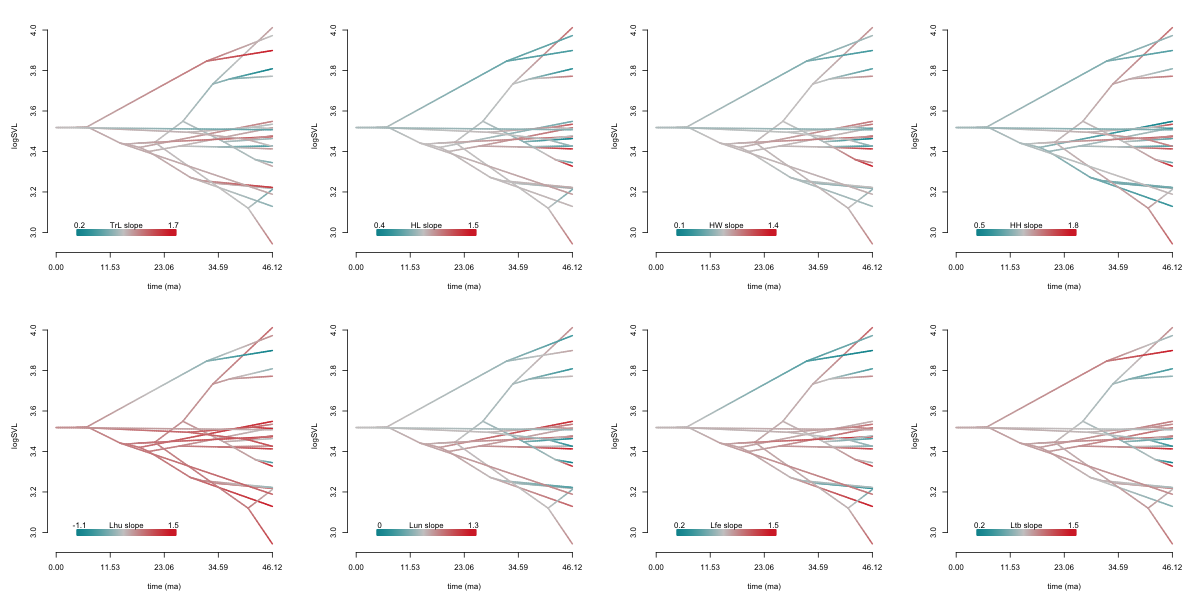
\includegraphics[width=0.9\linewidth]{Figs/phenograms_variables} 

}

\caption{Traitgrams of regression slopes for each phenotypic variable. Colors at the tips designate habitat groups.}\label{fig:unnamed-chunk-4}
\end{figure}

\newpage

\hypertarget{evolutionary-mapping-of-head-limb-allometry}{%
\subsubsection{Evolutionary Mapping of Head \& Limb
Allometry}\label{evolutionary-mapping-of-head-limb-allometry}}

In the main article, allometric trends in both head dimensions were
mapped onto the phylogeny under a Brownian motion model of evolution to
discern macroevolutionary changes across the phylogeny. These were
visualized on traitgrams, where body size differences were optimized
(main article: Fig. 3). Here we present evolutionary mappings of
allometric trends individually, so that increases and decreases in
allometric slopes across the phylogeny are more readily interpreted. A
summary of these patterns was described in the main article.

Briefly, these plots show that changes in allometry were not
concentrated to particular regions of the phylogeny, but rather
displayed both increases and decreases in allometry of both the head
traits and the limb traits occurred repeatedly in this group.

\begin{figure}[H]

{\centering 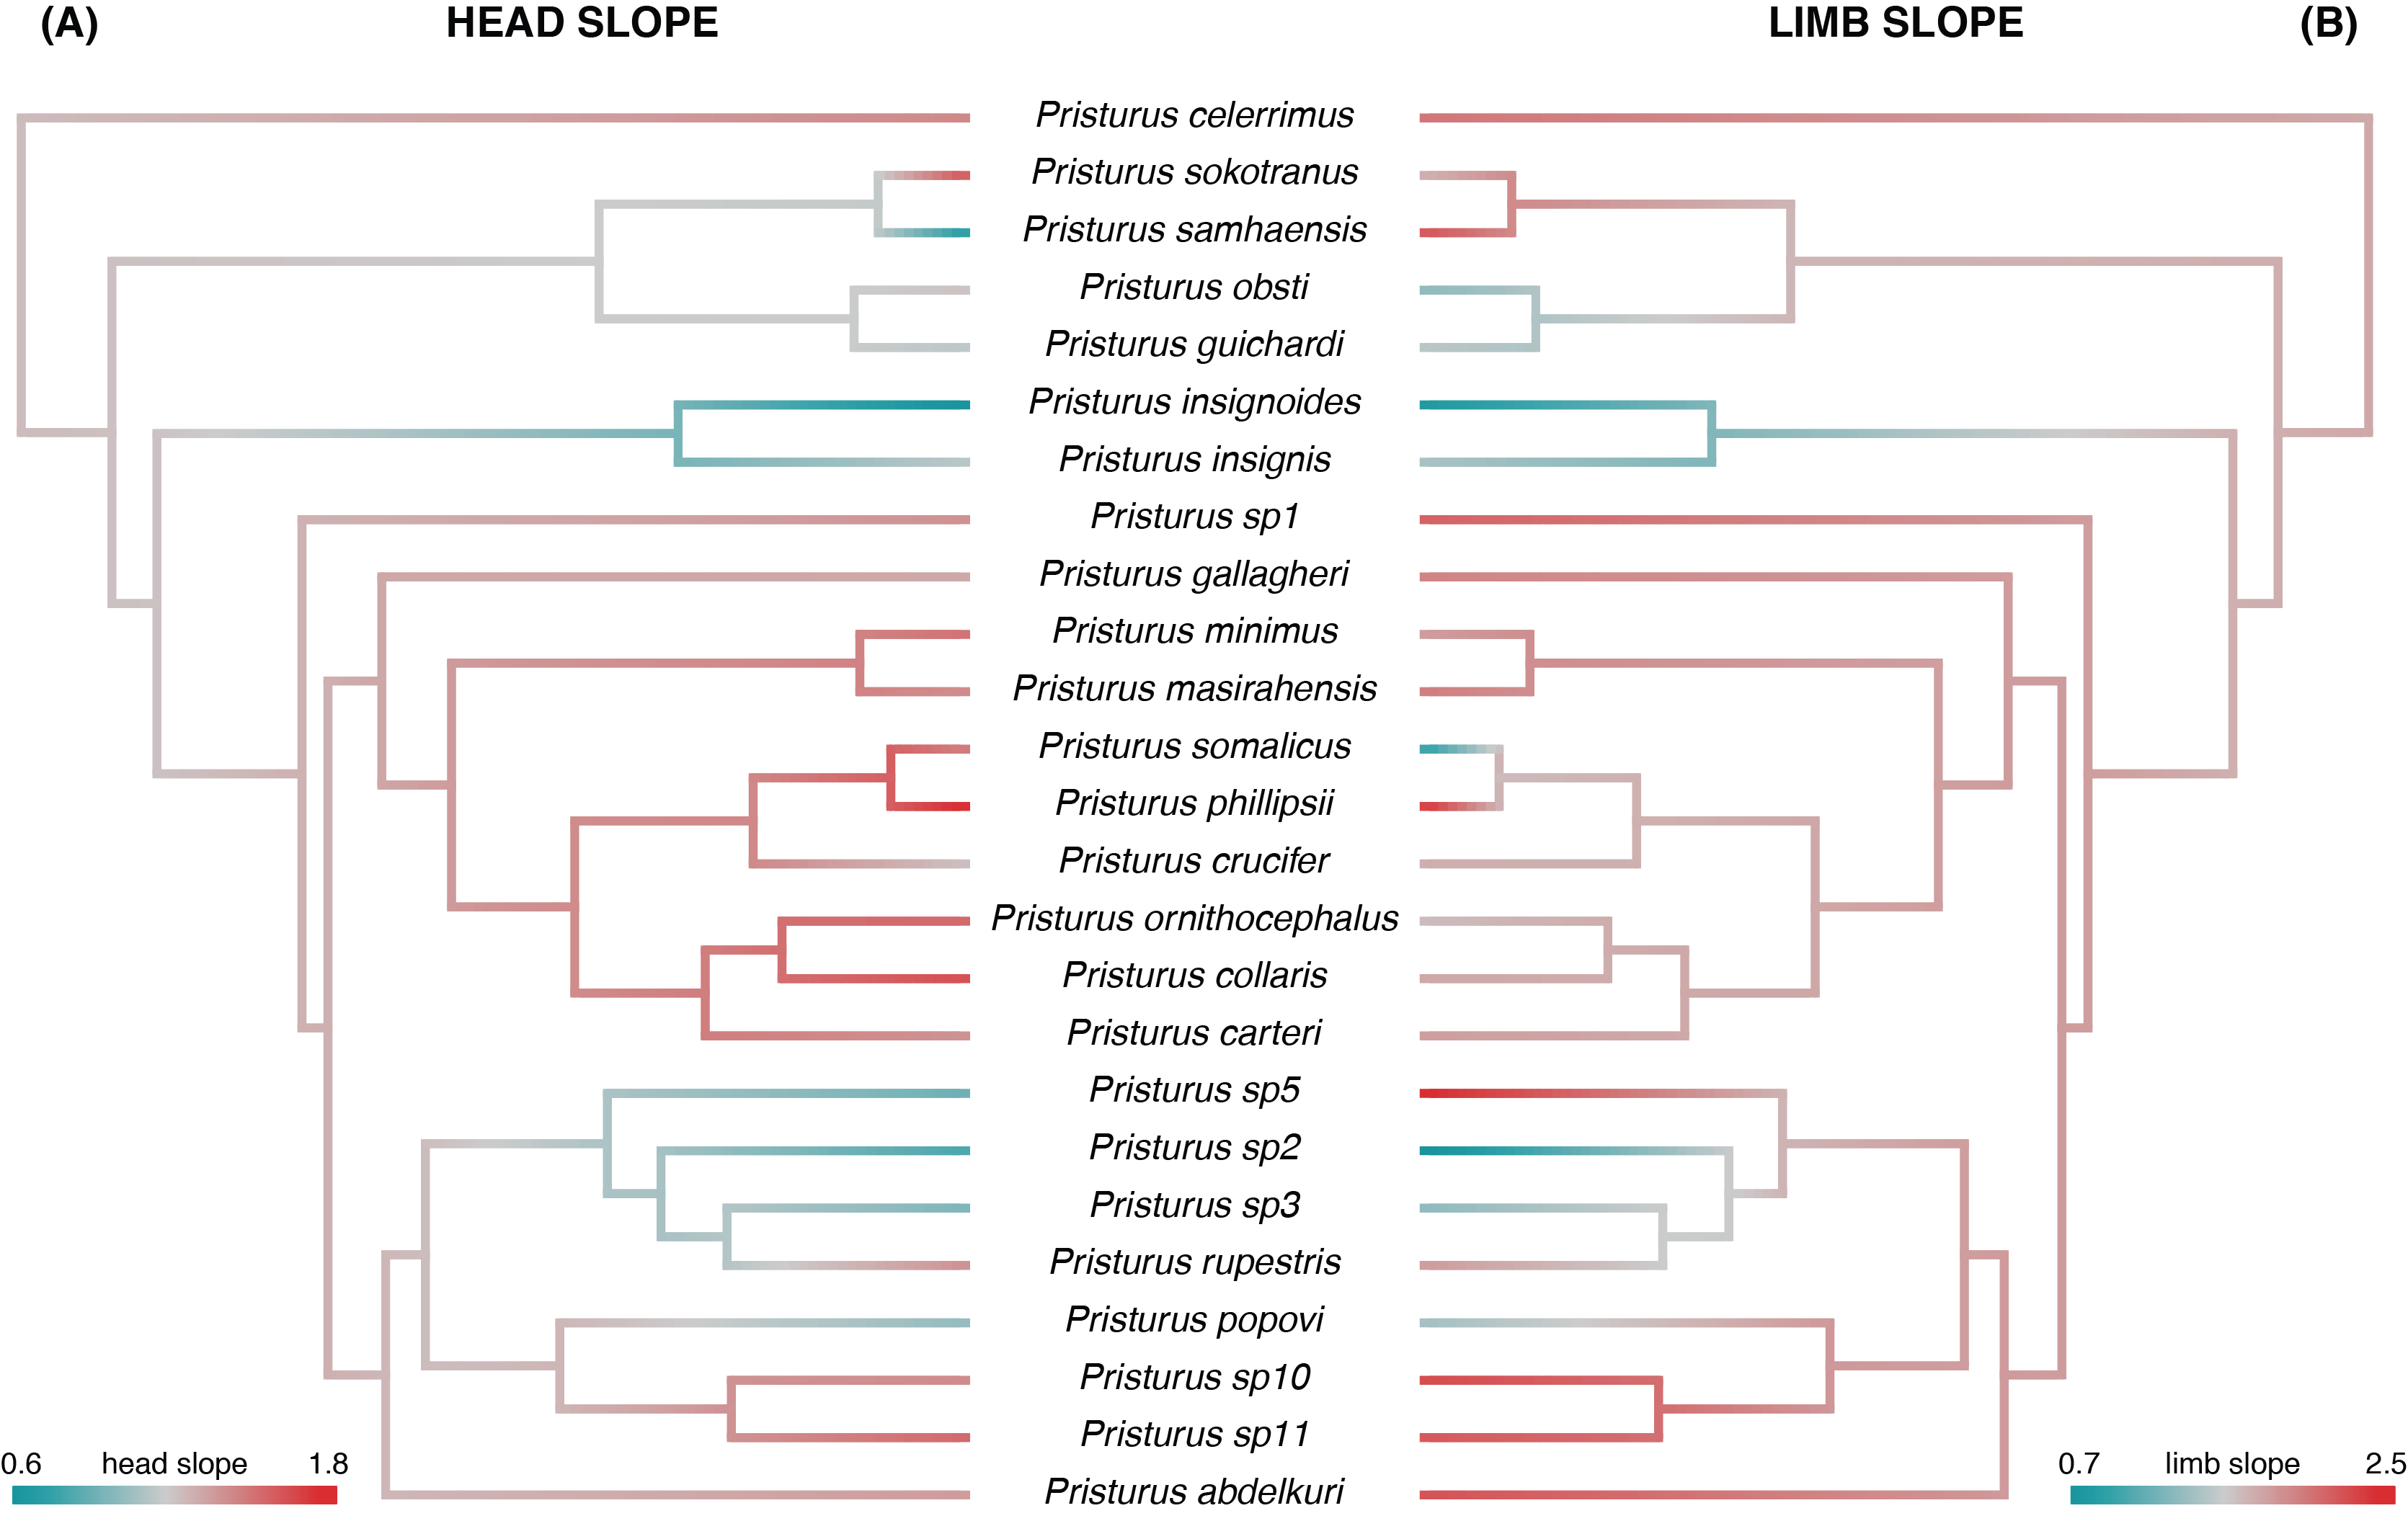
\includegraphics[width=1\linewidth]{Figs/contmap_slopes} 

}

\caption{Evolutionary mapping of regression slopes describing the relationship of (A) head morphology versus body size, and (B) limb proportions versus body size.}\label{fig:unnamed-chunk-5}
\end{figure}

\newpage

\hypertarget{morphological-integration}{%
\subsubsection{Morphological
Integration}\label{morphological-integration}}

In the main article, we performed analyses of morphological integration
on the set of body traits representing body form. Here we perform the
same analysis, using size-standardized data.

\begin{Shaded}
\begin{Highlighting}[]
\NormalTok{shape}\FloatTok{.2} \OtherTok{\textless{}{-}}\NormalTok{ shape }\SpecialCharTok{{-}}\NormalTok{ rdf}\SpecialCharTok{$}\NormalTok{svl}
\NormalTok{shape.gp }\OtherTok{\textless{}{-}} \FunctionTok{lapply}\NormalTok{( }\FunctionTok{split}\NormalTok{( shape}\FloatTok{.2}\NormalTok{[,}\DecValTok{1}\SpecialCharTok{:}\FunctionTok{ncol}\NormalTok{(shape}\FloatTok{.2}\NormalTok{)], rdf}\SpecialCharTok{$}\NormalTok{habitat), }
\NormalTok{                    matrix, }\AttributeTok{ncol=}\FunctionTok{ncol}\NormalTok{(shape}\FloatTok{.2}\NormalTok{))}
\NormalTok{Vrel.gp.shp }\OtherTok{\textless{}{-}} \FunctionTok{Map}\NormalTok{(}\ControlFlowTok{function}\NormalTok{(x) }\FunctionTok{integration.Vrel}\NormalTok{(x), shape.gp) }
\FunctionTok{c}\NormalTok{(Vrel.gp.shp}\SpecialCharTok{$}\NormalTok{ground}\SpecialCharTok{$}\NormalTok{ZR,Vrel.gp.shp}\SpecialCharTok{$}\NormalTok{rock}\SpecialCharTok{$}\NormalTok{ZR,Vrel.gp.shp}\SpecialCharTok{$}\NormalTok{tree}\SpecialCharTok{$}\NormalTok{ZR)}
\end{Highlighting}
\end{Shaded}

\begin{verbatim}
## [1] 2.403052 1.904412 1.224868
\end{verbatim}

\begin{Shaded}
\begin{Highlighting}[]
\NormalTok{out.shp }\OtherTok{\textless{}{-}} \FunctionTok{compare.ZVrel}\NormalTok{(Vrel.gp.shp}\SpecialCharTok{$}\NormalTok{ground, Vrel.gp.shp}\SpecialCharTok{$}\NormalTok{rock, Vrel.gp.shp}\SpecialCharTok{$}\NormalTok{tree)}
\FunctionTok{summary}\NormalTok{(out.shp)}
\end{Highlighting}
\end{Shaded}

\begin{verbatim}
## 
## Effect sizes
## 
## Vrel.gp.shp$ground   Vrel.gp.shp$rock   Vrel.gp.shp$tree 
##         -0.1468813         -0.9606380         -0.9189899 
## 
## Effect sizes for pairwise differences in rel.eig effect size
## 
##                    Vrel.gp.shp$ground Vrel.gp.shp$rock Vrel.gp.shp$tree
## Vrel.gp.shp$ground           0.000000        9.3926169        6.1015621
## Vrel.gp.shp$rock             9.392617        0.0000000        0.3556259
## Vrel.gp.shp$tree             6.101562        0.3556259        0.0000000
## 
## P-values
## 
##                    Vrel.gp.shp$ground Vrel.gp.shp$rock Vrel.gp.shp$tree
## Vrel.gp.shp$ground       1.000000e+00     5.852770e-21     1.050368e-09
## Vrel.gp.shp$rock         5.852770e-21     1.000000e+00     7.221208e-01
## Vrel.gp.shp$tree         1.050368e-09     7.221208e-01     1.000000e+00
\end{verbatim}

\newpage

\hypertarget{references}{%
\section*{References}\label{references}}
\addcontentsline{toc}{section}{References}

\setlength{\parindent}{-0.25in} \setlength{\leftskip}{0.25in}
\setlength{\parskip}{8pt} \noindent

\hypertarget{refs}{}
\begin{CSLReferences}{1}{0}
\leavevmode\vadjust pre{\hypertarget{ref-PristurusData}{}}%
Tejero-Cicuéndez, H., M. Simó-Riudalbas, I. Menéndez, and S. Carranza.
2021. Ecological specialization, rather than the island effect, explains
morphological diversification in an ancient radiation of geckos. Dryad
digital repository. (Doi:10.5061/dryad.xwdbrv1f6).

\end{CSLReferences}

\newpage

\end{document}
